\section{若干湍流模型的数值比较}
\label{sec:comparison-turbulence-models}

\begin{note}[内容]
\label{note:comparison-turbulence-models-contents}
本节比较本章介绍的若干湍流模型所得到的数值解.重点讨论 Smagorinsky 模型和三尺度粗空间投影 VMS 方法,因为在 $\mathrm{Re}_\tau=180$ 的湍流槽道流中,这两种方法给出的结果最准确.对本节涉及的问题,采用有理 LES 模型、Leray-$\alpha$ 模型和 Navier--Stokes-$\alpha$ 模型进行模拟,通常无法得到令人满意的结果.
\end{note}

\begin{example}[($\mathrm{Re}_\tau=180$ 的湍流槽道流)]
\label{ex:vms-comparison-channel-180}
本例仅列出例题\hyperref[ex:smagorinsky-turbulent-channel]{8.128}和\hyperref[ex:vms-coarse-projection-channel-flow]{8.277}中所考察湍流模型的最佳参数:
\begin{itemize}
 \item Smagorinsky 模型\hyperref[eq:smagorinsky-filter-width]{(8.69)}(Smag):$\delta_K=2h_{K,\mathrm{short}}$,$C_S=0.005$,并采用 van Driest 阻尼\hyperref[eq:van-driest-damping]{(8.152)};
 \item 粗空间投影方法\hyperref[eq:vms-coarse-projection-three-scale-method]{(8.288)},其中 $\mathcal L^H=\mathbb P_0$(VMS0):$\delta_K=2h_{K,\mathrm{short}}$,$C_S=0.01$,不采用 van Driest 阻尼;
 \item 粗空间投影方法\hyperref[eq:vms-coarse-projection-three-scale-method]{(8.288)},其中 $\mathcal L^H=\mathbb P_1^{\mathrm{disc}}$(VMS1):$\delta_K=2h_{K,\mathrm{short}}$,$C_S=0.02$,不采用 van Driest 阻尼;
 \item 自适应选取投影空间的粗空间投影方法(VMSadap):$\delta_K=2h_{K,\mathrm{short}}$,$C_S=0.02$,并采用 van Driest 阻尼\hyperref[eq:van-driest-damping]{(8.152)}.
\end{itemize}
这些参数下的结果见图\hyperref[fig:vms-comparison-channel-180]{8.14}.在所比较的湍流模型中,VMS0 和 VMSadap 的结果最准确,而 Smagorinsky 模型的结果最不准确.

\begin{elegantfigure}[333.25pt]
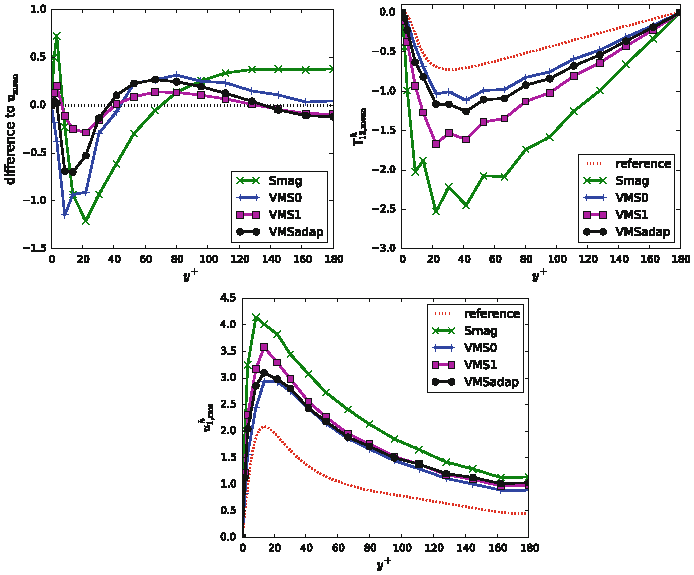
\includegraphics[width=333.25pt]{figures/Chapter_08/Fig_8_14__PDFp651__Bookp642.pdf}
\captionof{figure}{例题\hyperref[ex:vms-comparison-channel-180]{8.279}:$\mathrm{Re}_\tau=180$ 湍流槽道流中,Smagorinsky 模型和三尺度粗空间投影 VMS 模型采用最佳参数时的若干统计量.}
\label{fig:vms-comparison-channel-180}
\end{elegantfigure}
\end{example}

\begin{example}[($\mathrm{Re}_\tau=395$ 的湍流槽道流)]
\label{ex:vms-comparison-channel-395}
本例的说明见例题\hyperref[ex:appendix-d-12]{D.12}.模拟设置与 $\mathrm{Re}_\tau=180$ 的湍流槽道流相似,参见例题\hyperref[ex:smagorinsky-turbulent-channel]{8.128},只是空间网格和时间步长更细.空间网格由 $16\times16\times32$ 个单元组成.对 $Q_2/\mathbb P_1^{\mathrm{disc}}$ 有限元空间对,速度自由度为 199,680 个(包括 Dirichlet 节点),压力自由度为 32,768 个.Crank--Nicolson 格式的时间步长取 $\Delta t=0.002$.时间区间长度、靠近壁面的网格加密等其他设置均与例题\hyperref[ex:smagorinsky-turbulent-channel]{8.128}相同.

结果见图\hyperref[fig:vms-comparison-channel-395]{8.15}.VMS0 配合 $C_S=0.02$ 得到的结果最好.Smagorinsky 模型取 $C_S=0.01$、VMSadap 取 $C_S=0.02$ 时,也得到同样较好的结果.VMS1 取 $C_S=0.01$、Smagorinsky 模型取 $C_S=0.005$ 时,结果不准确.因此,针对 $\mathrm{Re}_\tau=180$ 湍流槽道流选出的 Smagorinsky 模型最佳参数,并不适用于本例.

\begin{elegantfigure}[333.5pt]
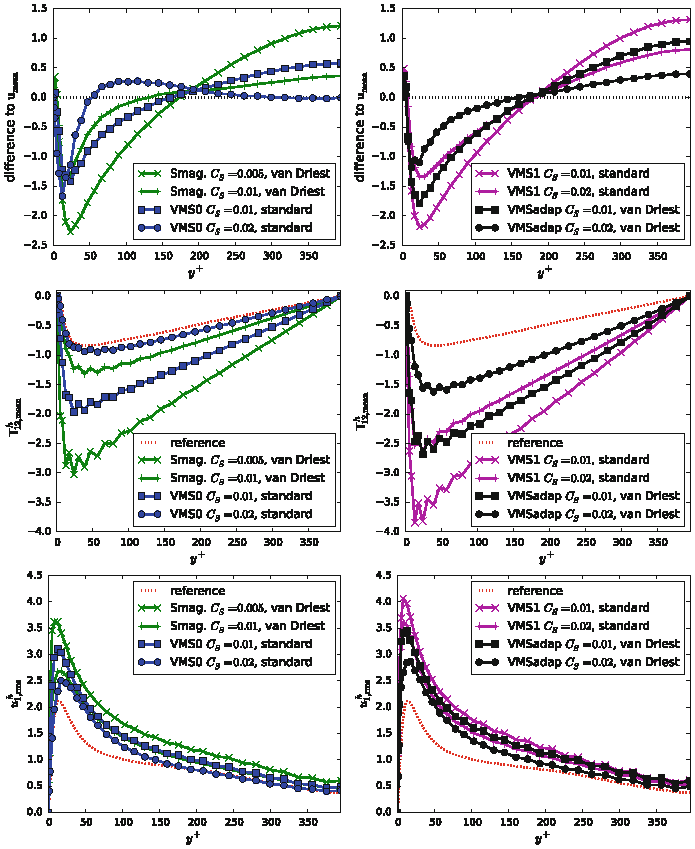
\includegraphics[width=333.5pt]{figures/Chapter_08/Fig_8_15__PDFp652__Bookp643.pdf}
\captionof{figure}{例题\hyperref[ex:vms-comparison-channel-395]{8.280}:$\mathrm{Re}_\tau=395$ 湍流槽道流中,Smagorinsky 模型和三尺度粗空间投影 VMS 模型所得的若干统计量.}
\label{fig:vms-comparison-channel-395}
\end{elegantfigure}
\end{example}

\begin{example}[($\mathrm{Re}=22{,}000$ 的绕圆柱湍流)]
\label{ex:vms-comparison-cylinder}
本例及其关注量见例题\hyperref[ex:appendix-d-13]{D.13}.模拟采用六面体网格和 $Q_2/\mathbb P_1^{\mathrm{disc}}$ 空间对;在第 2 层网格上,速度自由度为 522,720 个(包括 Dirichlet 节点),压力自由度为 81,920 个.图\hyperref[fig:vms-comparison-cylinder-grid]{8.16}给出了初始网格(第 0 层).时间离散采用等距步长 $\Delta t=0.005$ 的 Crank--Nicolson 格式.

\begin{elegantfigure}[226.5pt]
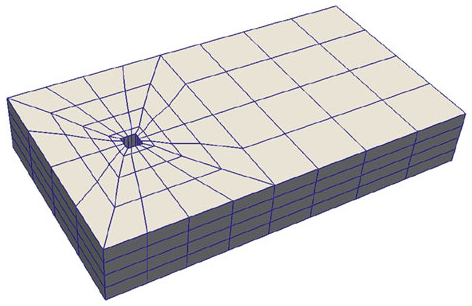
\includegraphics[width=226.5pt]{figures/Chapter_08/Fig_8_16__PDFp653__Bookp644.pdf}
\captionof{figure}{例题\hyperref[ex:vms-comparison-cylinder]{8.281}:初始网格,第 0 层.}
\label{fig:vms-comparison-cylinder-grid}
\end{elegantfigure}

本例不采用 van Driest 阻尼.所有流动均先发展 10 秒,随后在 30 个周期内计算统计量.

\begin{eleganttable}
\centering
\captionof{table}{例题\hyperref[ex:vms-comparison-cylinder]{8.281}}
\label{tab:vms-comparison-cylinder-statistics}
\scriptsize
\setlength{\tabcolsep}{2.5pt}
\renewcommand{\arraystretch}{1.16}
\resizebox{\linewidth}{!}{%
\begin{tabular}{l|c|cc|cc|c}
\hline
方法 & $C_S$ & $c_{\mathrm{lift}}$ & $c_{\mathrm{lift,rms}}$
 & $c_{\mathrm{drag}}$ & $c_{\mathrm{drag,rms}}$ & $\mathrm{St}$\\
\hline
Smag & 0.005 & \multicolumn{5}{c}{计算发散}\\
Smag & 0.01 & 0.001 & 1.46 & 2.58 & 0.11 & 0.151\\
Smag & 0.02 & 0.023 & 1.52 & 2.52 & 0.16 & 0.140\\
VMS0 & 0.01 & $-0.017$ & 1.28 & 2.60 & 0.19 & 0.139\\
VMS0 & 0.02 & $-0.015$ & 1.29 & 2.65 & 0.14 & 0.142\\
VMS1 & 0.01 & $-0.004$ & 1.04 & 2.49 & 0.15 & 0.136\\
VMS1 & 0.02 & $-0.026$ & 1.00 & 2.50 & 0.21 & 0.131\\
VMSadap & 0.01 & $-0.006$ & 1.15 & 2.49 & 0.21 & 0.131\\
VMSadap & 0.02 & $-0.026$ & 1.49 & 2.55 & 0.16 & 0.141\\
实验值 & & 0 & $[0.7,1.4]$ & $[1.9,2.1]$ & $[0.1,0.2]$ & 0.132\\
\hline
\end{tabular}%
}
\par\smallskip
\footnotesize 关注量的计算值及实验值.
\end{eleganttable}

表\hyperref[tab:vms-comparison-cylinder-statistics]{8.1}列出了所比较方法得到的结果.大多数结果在定性上相近:均方根(rms)值处于实验区间内,或仅略微超出该区间;平均阻力系数则明显高于实验值.文献中也经常报告后一现象,例如\textcite{GravemeierKronbichlerGeeWall2011,RasthoferGravemeier2013}.各方法所得 Strouhal 数之间则存在较明显差异:Smagorinsky 模型取 $C_S=0.01$ 时结果最差,VMS1 的结果最好.

\begin{elegantfigure}[226.5pt]
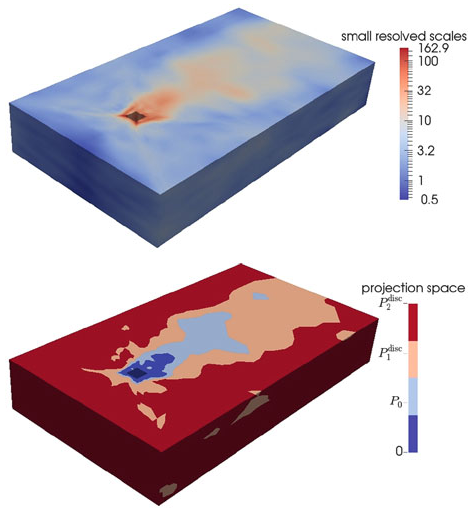
\includegraphics[width=226.5pt]{figures/Chapter_08/Fig_8_17__PDFp654__Bookp645.pdf}
\captionof{figure}{例题\hyperref[ex:vms-comparison-cylinder]{8.281}:自适应投影空间的三尺度投影 VMS 方法中,小的已解析尺度的大小(上)及相应投影空间(下).}
\label{fig:vms-adaptive-cylinder-flow}
\end{elegantfigure}

此外,Smagorinsky 模型取 $C_S=0.005$ 时发散,这一点值得注意.因此,该模型在 $\mathrm{Re}_\tau=180$ 湍流槽道流中的最佳参数在本例中失效.相较之下,本例也表明三尺度粗空间投影 VMS 方法对 $C_S$ 的选取不那么敏感.

图\hyperref[fig:vms-adaptive-cylinder-flow]{8.17}展示了小的已解析尺度的大小、空间分布以及自适应投影空间的相应选取.本例中,圆柱表面及其下游区域的湍流强度预计最高.图中小的已解析尺度的大小与这一预期相符,因此式\hyperref[eq:vms-coarse-projection-local-turbulence-intensity]{(8.328)}中的 $\zeta_K$ 是合适的局部湍流强度估计量.从投影空间图中可以看出,湍流模型在圆柱处的影响最大,沿下游方向逐渐减弱,在其他区域则基本关闭.
\end{example}

\begin{example}[($\mathrm{Re}=40{,}000$ 的壁装立方体绕流)]
\label{ex:vms-comparison-wall-mounted-cube}
本问题见例题\hyperref[ex:appendix-d-14]{D.14}.

\begin{elegantfigure}[226.5pt]
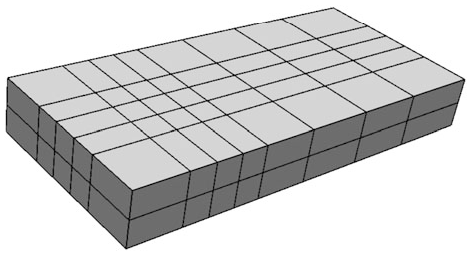
\includegraphics[width=226.5pt]{figures/Chapter_08/Fig_8_18__PDFp655__Bookp646.pdf}
\captionof{figure}{例题\hyperref[ex:vms-comparison-wall-mounted-cube]{8.282}:初始网格,第 0 层.}
\label{fig:vms-comparison-wall-mounted-cube-grid}
\end{elegantfigure}

数值模拟采用六面体网格上的 $Q_2/\mathbb P_1^{\mathrm{disc}}$ 空间对.初始网格(第 0 层)见图\hyperref[fig:vms-comparison-wall-mounted-cube-grid]{8.18},表\hyperref[tab:vms-comparison-wall-mounted-cube-dofs]{8.2}列出了自由度数量.模拟时间区间为 $[0,10]$,时间离散采用等距步长 $\Delta t=0.01$ 的 Crank--Nicolson 格式.计算阻力系数的时间平均值时,取区间 $[5,10]$.所有湍流模型均未采用 van Driest 阻尼.

\begin{eleganttable}[0.68\linewidth]
\centering
\captionof{table}{例题\hyperref[ex:vms-comparison-wall-mounted-cube]{8.282}}
\label{tab:vms-comparison-wall-mounted-cube-dofs}
\scriptsize
\setlength{\tabcolsep}{4pt}
\renewcommand{\arraystretch}{1.12}
\begin{tabular}{c|rrr}
\hline
层级 & 速度 & 压力 & 总计\\
\hline
2 & 134,739 & 20,224 & 154,963\\
3 & 1,023,651 & 161,792 & 1,185,443\\
\hline
\end{tabular}
\par\smallskip
\footnotesize 空间自由度数(包括 Dirichlet 节点).
\end{eleganttable}

\begin{eleganttable}[0.82\linewidth]
\centering
\captionof{table}{例题\hyperref[ex:vms-comparison-wall-mounted-cube]{8.282}}
\label{tab:vms-comparison-wall-mounted-cube-drag}
\scriptsize
\setlength{\tabcolsep}{4pt}
\renewcommand{\arraystretch}{1.12}
\begin{tabular}{l|c|cc}
\hline
方法 & $C_S$ & 第 2 层 & 第 3 层\\
\hline
Smag & 0.005 & 1.16 & 1.46\\
Smag & 0.01 & 1.26 & 1.45\\
VMS0 & 0.01 & 1.19 & 1.47\\
VMS0 & 0.02 & 1.23 & 1.45\\
VMS1 & 0.01 & 1.09 & 1.39\\
VMS1 & 0.02 & 1.11 & 1.38\\
VMSadap & 0.01 & 1.13 & 1.37\\
VMSadap & 0.02 & 1.21 & 1.33\\
\hline
\end{tabular}
\par\smallskip
\footnotesize 平均阻力系数;参考值 $c_{\mathrm{drag}}\approx1.5$.
\end{eleganttable}

表\hyperref[tab:vms-comparison-wall-mounted-cube-drag]{8.3}给出了不同湍流模型的结果.图\hyperref[fig:vms-comparison-wall-mounted-cube-drag]{8.19}以两种模型为例,展示了计算所得阻力系数随时间的变化.可以看到,所有湍流模型在较粗的第 2 层网格上都低估了平均阻力系数.在较细的第 3 层网格上,Smagorinsky 模型和 VMS0 所得平均阻力系数与参考值处于同一量级;VMS1 和 VMSadap 仍明显低估这一系数.图\hyperref[fig:vms-comparison-wall-mounted-cube-drag]{8.19}还表明,在较细网格上,计算阻力系数围绕其平均值的振荡幅度显著减小.

\begin{elegantfigure}[333.25pt]
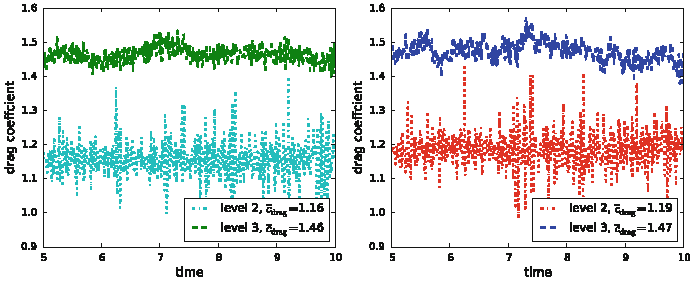
\includegraphics[width=333.25pt]{figures/Chapter_08/Fig_8_19__PDFp656__Bookp647.pdf}
\captionof{figure}{例题\hyperref[ex:vms-comparison-wall-mounted-cube]{8.282}:Smagorinsky 模型 $C_S=0.005$(左)和 VMS0 $C_S=0.01$(右)所得阻力系数.}
\label{fig:vms-comparison-wall-mounted-cube-drag}
\end{elegantfigure}
\end{example}

\index{湍流模型!数值比较}
\index{Smagorinsky 模型!与 VMS 方法比较}
\index{变分多尺度方法!基于粗空间投影!数值比较}
